% Options for packages loaded elsewhere
\PassOptionsToPackage{unicode}{hyperref}
\PassOptionsToPackage{hyphens}{url}
\PassOptionsToPackage{dvipsnames,svgnames,x11names}{xcolor}
%
\documentclass[
]{article}
\usepackage{amsmath,amssymb}
\usepackage{iftex}
\ifPDFTeX
  \usepackage[T1]{fontenc}
  \usepackage[utf8]{inputenc}
  \usepackage{textcomp} % provide euro and other symbols
\else % if luatex or xetex
  \usepackage{unicode-math} % this also loads fontspec
  \defaultfontfeatures{Scale=MatchLowercase}
  \defaultfontfeatures[\rmfamily]{Ligatures=TeX,Scale=1}
\fi
\usepackage{lmodern}
\ifPDFTeX\else
  % xetex/luatex font selection
\fi
% Use upquote if available, for straight quotes in verbatim environments
\IfFileExists{upquote.sty}{\usepackage{upquote}}{}
\IfFileExists{microtype.sty}{% use microtype if available
  \usepackage[]{microtype}
  \UseMicrotypeSet[protrusion]{basicmath} % disable protrusion for tt fonts
}{}
\makeatletter
\@ifundefined{KOMAClassName}{% if non-KOMA class
  \IfFileExists{parskip.sty}{%
    \usepackage{parskip}
  }{% else
    \setlength{\parindent}{0pt}
    \setlength{\parskip}{6pt plus 2pt minus 1pt}}
}{% if KOMA class
  \KOMAoptions{parskip=half}}
\makeatother
\usepackage{xcolor}
\usepackage[margin=1in]{geometry}
\usepackage{color}
\usepackage{fancyvrb}
\newcommand{\VerbBar}{|}
\newcommand{\VERB}{\Verb[commandchars=\\\{\}]}
\DefineVerbatimEnvironment{Highlighting}{Verbatim}{commandchars=\\\{\}}
% Add ',fontsize=\small' for more characters per line
\usepackage{framed}
\definecolor{shadecolor}{RGB}{248,248,248}
\newenvironment{Shaded}{\begin{snugshade}}{\end{snugshade}}
\newcommand{\AlertTok}[1]{\textcolor[rgb]{0.94,0.16,0.16}{#1}}
\newcommand{\AnnotationTok}[1]{\textcolor[rgb]{0.56,0.35,0.01}{\textbf{\textit{#1}}}}
\newcommand{\AttributeTok}[1]{\textcolor[rgb]{0.13,0.29,0.53}{#1}}
\newcommand{\BaseNTok}[1]{\textcolor[rgb]{0.00,0.00,0.81}{#1}}
\newcommand{\BuiltInTok}[1]{#1}
\newcommand{\CharTok}[1]{\textcolor[rgb]{0.31,0.60,0.02}{#1}}
\newcommand{\CommentTok}[1]{\textcolor[rgb]{0.56,0.35,0.01}{\textit{#1}}}
\newcommand{\CommentVarTok}[1]{\textcolor[rgb]{0.56,0.35,0.01}{\textbf{\textit{#1}}}}
\newcommand{\ConstantTok}[1]{\textcolor[rgb]{0.56,0.35,0.01}{#1}}
\newcommand{\ControlFlowTok}[1]{\textcolor[rgb]{0.13,0.29,0.53}{\textbf{#1}}}
\newcommand{\DataTypeTok}[1]{\textcolor[rgb]{0.13,0.29,0.53}{#1}}
\newcommand{\DecValTok}[1]{\textcolor[rgb]{0.00,0.00,0.81}{#1}}
\newcommand{\DocumentationTok}[1]{\textcolor[rgb]{0.56,0.35,0.01}{\textbf{\textit{#1}}}}
\newcommand{\ErrorTok}[1]{\textcolor[rgb]{0.64,0.00,0.00}{\textbf{#1}}}
\newcommand{\ExtensionTok}[1]{#1}
\newcommand{\FloatTok}[1]{\textcolor[rgb]{0.00,0.00,0.81}{#1}}
\newcommand{\FunctionTok}[1]{\textcolor[rgb]{0.13,0.29,0.53}{\textbf{#1}}}
\newcommand{\ImportTok}[1]{#1}
\newcommand{\InformationTok}[1]{\textcolor[rgb]{0.56,0.35,0.01}{\textbf{\textit{#1}}}}
\newcommand{\KeywordTok}[1]{\textcolor[rgb]{0.13,0.29,0.53}{\textbf{#1}}}
\newcommand{\NormalTok}[1]{#1}
\newcommand{\OperatorTok}[1]{\textcolor[rgb]{0.81,0.36,0.00}{\textbf{#1}}}
\newcommand{\OtherTok}[1]{\textcolor[rgb]{0.56,0.35,0.01}{#1}}
\newcommand{\PreprocessorTok}[1]{\textcolor[rgb]{0.56,0.35,0.01}{\textit{#1}}}
\newcommand{\RegionMarkerTok}[1]{#1}
\newcommand{\SpecialCharTok}[1]{\textcolor[rgb]{0.81,0.36,0.00}{\textbf{#1}}}
\newcommand{\SpecialStringTok}[1]{\textcolor[rgb]{0.31,0.60,0.02}{#1}}
\newcommand{\StringTok}[1]{\textcolor[rgb]{0.31,0.60,0.02}{#1}}
\newcommand{\VariableTok}[1]{\textcolor[rgb]{0.00,0.00,0.00}{#1}}
\newcommand{\VerbatimStringTok}[1]{\textcolor[rgb]{0.31,0.60,0.02}{#1}}
\newcommand{\WarningTok}[1]{\textcolor[rgb]{0.56,0.35,0.01}{\textbf{\textit{#1}}}}
\usepackage{longtable,booktabs,array}
\usepackage{calc} % for calculating minipage widths
% Correct order of tables after \paragraph or \subparagraph
\usepackage{etoolbox}
\makeatletter
\patchcmd\longtable{\par}{\if@noskipsec\mbox{}\fi\par}{}{}
\makeatother
% Allow footnotes in longtable head/foot
\IfFileExists{footnotehyper.sty}{\usepackage{footnotehyper}}{\usepackage{footnote}}
\makesavenoteenv{longtable}
\usepackage{graphicx}
\makeatletter
\def\maxwidth{\ifdim\Gin@nat@width>\linewidth\linewidth\else\Gin@nat@width\fi}
\def\maxheight{\ifdim\Gin@nat@height>\textheight\textheight\else\Gin@nat@height\fi}
\makeatother
% Scale images if necessary, so that they will not overflow the page
% margins by default, and it is still possible to overwrite the defaults
% using explicit options in \includegraphics[width, height, ...]{}
\setkeys{Gin}{width=\maxwidth,height=\maxheight,keepaspectratio}
% Set default figure placement to htbp
\makeatletter
\def\fps@figure{htbp}
\makeatother
\setlength{\emergencystretch}{3em} % prevent overfull lines
\providecommand{\tightlist}{%
  \setlength{\itemsep}{0pt}\setlength{\parskip}{0pt}}
\setcounter{secnumdepth}{5}
\usepackage{fvextra} \DefineVerbatimEnvironment{Highlighting}{Verbatim}{breaklines,commandchars=\\\{\}}
\ifLuaTeX
  \usepackage{selnolig}  % disable illegal ligatures
\fi
\usepackage{bookmark}
\IfFileExists{xurl.sty}{\usepackage{xurl}}{} % add URL line breaks if available
\urlstyle{same}
\hypersetup{
  pdftitle={Surrogate Splits with SMOTE},
  colorlinks=true,
  linkcolor={Maroon},
  filecolor={Maroon},
  citecolor={Blue},
  urlcolor={blue},
  pdfcreator={LaTeX via pandoc}}

\title{Surrogate Splits with SMOTE}
\author{}
\date{\vspace{-2.5em}}

\begin{document}
\maketitle

{
\hypersetup{linkcolor=}
\setcounter{tocdepth}{2}
\tableofcontents
}
\section{Introduction}\label{introduction}

We got a very weak specificity in the previous model. Treating missingness on its own was not enough to get a good performance. We therefore look at how to deal with the imbalance.

In the literature, many methods have been devised to address imbalanced data. These can be grouped into 3 main categories {[}Chapter 5, 1{]}:

\begin{itemize}
\tightlist
\item
  \textbf{Sampling methods:} The training set is modified to produce a more balanced distribution that allows classifiers to perform in a similar manner to standard classification. These methods are sometimes called data-level modifications.
\item
  \textbf{Algorithm-level modifications:} The classification algorithm is modified to be more attuned to class imbalance.
\item
  \textbf{Cost-sensitive learning:} This incorporates data-level and algorithm-level modifications by considering variable misclassification costs.
\end{itemize}

We will not have time to look into all of these, so we will only look at sampling methods. We refer the reader to the book cited for more details.

\section{Details behind SMOTE}\label{details-behind-smote}

We discuss one sampling method called the \textit{Synthetic Minority Oversampling Technique} (SMOTE). It is based on the creation of synthetic data by interpolating between minority samples using their nearest neighbours (see the KNN classifier for how we define neighbours). Note that we encode each feature \(\boldsymbol{x}\) so that each \(x_i \in \mathbb{R}\) so that interpolation is possible. The formal process works as follows, and is adapted from {[}Chapter 5.4, 1{]}. First, an integer value \(N\), the oversampling factor, is specified. Default behaviour in programs will usually choose this to balance the class distribution. Then, an iterative process is carried out. First, a minority class point \(\boldsymbol{x}^*\) is selected at random from the training set. Next, its \(K\) nearest neighbours are obtained. Finally, \(N\) of these \(K\) instances are randomly chosen (with repetitions allowed). Then, \(N\) synthetic examples are created by random linear interpolation between \(\boldsymbol{x}^*\) and each of the chosen nearest neighbours.

\section{Prerequisites}\label{prerequisites}

We load the SMOTE data using the code below.

\begin{Shaded}
\begin{Highlighting}[]
\CommentTok{\# List of required packages}
\NormalTok{packages }\OtherTok{\textless{}{-}} \FunctionTok{c}\NormalTok{(}\StringTok{"rpart"}\NormalTok{, }\StringTok{"caret"}\NormalTok{, }\StringTok{"pROC"}\NormalTok{, }\StringTok{"ggplot2"}\NormalTok{, }\StringTok{"dplyr"}\NormalTok{)}

\CommentTok{\# Install missing packages}
\NormalTok{install\_if\_missing }\OtherTok{\textless{}{-}} \ControlFlowTok{function}\NormalTok{(pkg) \{}
  \ControlFlowTok{if}\NormalTok{ (}\SpecialCharTok{!}\FunctionTok{require}\NormalTok{(pkg, }\AttributeTok{character.only =} \ConstantTok{TRUE}\NormalTok{)) \{}
    \FunctionTok{install.packages}\NormalTok{(pkg, }\AttributeTok{dependencies =} \ConstantTok{TRUE}\NormalTok{)}
\NormalTok{  \}}
\NormalTok{\}}

\CommentTok{\# Check and install missing packages}
\FunctionTok{invisible}\NormalTok{(}\FunctionTok{lapply}\NormalTok{(packages, install\_if\_missing))}
\end{Highlighting}
\end{Shaded}

\begin{verbatim}
## Loading required package: rpart
\end{verbatim}

\begin{verbatim}
## Loading required package: caret
\end{verbatim}

\begin{verbatim}
## Loading required package: ggplot2
\end{verbatim}

\begin{verbatim}
## Loading required package: lattice
\end{verbatim}

\begin{verbatim}
## Loading required package: pROC
\end{verbatim}

\begin{verbatim}
## Type 'citation("pROC")' for a citation.
\end{verbatim}

\begin{verbatim}
## 
## Attaching package: 'pROC'
\end{verbatim}

\begin{verbatim}
## The following objects are masked from 'package:stats':
## 
##     cov, smooth, var
\end{verbatim}

\begin{verbatim}
## Loading required package: dplyr
\end{verbatim}

\begin{verbatim}
## 
## Attaching package: 'dplyr'
\end{verbatim}

\begin{verbatim}
## The following objects are masked from 'package:stats':
## 
##     filter, lag
\end{verbatim}

\begin{verbatim}
## The following objects are masked from 'package:base':
## 
##     intersect, setdiff, setequal, union
\end{verbatim}

\begin{Shaded}
\begin{Highlighting}[]
\CommentTok{\# Load the packages}
\FunctionTok{lapply}\NormalTok{(packages, library, }\AttributeTok{character.only =} \ConstantTok{TRUE}\NormalTok{)}
\end{Highlighting}
\end{Shaded}

\begin{verbatim}
## [[1]]
##  [1] "dplyr"     "pROC"      "caret"     "lattice"   "ggplot2"   "rpart"    
##  [7] "stats"     "graphics"  "grDevices" "utils"     "datasets"  "methods"  
## [13] "base"     
## 
## [[2]]
##  [1] "dplyr"     "pROC"      "caret"     "lattice"   "ggplot2"   "rpart"    
##  [7] "stats"     "graphics"  "grDevices" "utils"     "datasets"  "methods"  
## [13] "base"     
## 
## [[3]]
##  [1] "dplyr"     "pROC"      "caret"     "lattice"   "ggplot2"   "rpart"    
##  [7] "stats"     "graphics"  "grDevices" "utils"     "datasets"  "methods"  
## [13] "base"     
## 
## [[4]]
##  [1] "dplyr"     "pROC"      "caret"     "lattice"   "ggplot2"   "rpart"    
##  [7] "stats"     "graphics"  "grDevices" "utils"     "datasets"  "methods"  
## [13] "base"     
## 
## [[5]]
##  [1] "dplyr"     "pROC"      "caret"     "lattice"   "ggplot2"   "rpart"    
##  [7] "stats"     "graphics"  "grDevices" "utils"     "datasets"  "methods"  
## [13] "base"
\end{verbatim}

\begin{Shaded}
\begin{Highlighting}[]
\CommentTok{\# rpart      {-} Recursive partitioning for decision trees}
\CommentTok{\# caret      {-} For confusion matrix and precision/recall calculations}
\CommentTok{\# pROC       {-} For ROC curve calculations}
\CommentTok{\# ggplot2    {-} For plotting}
\CommentTok{\# dplyr      {-} For data manipulation}

\CommentTok{\# Get the current working directory}
\NormalTok{current\_dir }\OtherTok{\textless{}{-}} \FunctionTok{getwd}\NormalTok{()}
\FunctionTok{cat}\NormalTok{(}\StringTok{"Current directory:"}\NormalTok{, current\_dir, }\StringTok{"}\SpecialCharTok{\textbackslash{}n}\StringTok{"}\NormalTok{)}
\end{Highlighting}
\end{Shaded}

\begin{verbatim}
## Current directory: C:/Users/megar/Documents/Code/Data Science Toolbox/dst-group-project-1/VivekP
\end{verbatim}

\begin{Shaded}
\begin{Highlighting}[]
\CommentTok{\# Get the parent directory}
\NormalTok{parent\_dir }\OtherTok{\textless{}{-}} \FunctionTok{dirname}\NormalTok{(current\_dir)}
\FunctionTok{cat}\NormalTok{(}\StringTok{"Parent directory:"}\NormalTok{, parent\_dir, }\StringTok{"}\SpecialCharTok{\textbackslash{}n}\StringTok{"}\NormalTok{)}
\end{Highlighting}
\end{Shaded}

\begin{verbatim}
## Parent directory: C:/Users/megar/Documents/Code/Data Science Toolbox/dst-group-project-1
\end{verbatim}

\begin{Shaded}
\begin{Highlighting}[]
\CommentTok{\# Set the working directory to the parent directory}
\FunctionTok{setwd}\NormalTok{(parent\_dir)}
\FunctionTok{cat}\NormalTok{(}\StringTok{"New working directory:"}\NormalTok{, }\FunctionTok{getwd}\NormalTok{(), }\StringTok{"}\SpecialCharTok{\textbackslash{}n}\StringTok{"}\NormalTok{)}
\end{Highlighting}
\end{Shaded}

\begin{verbatim}
## New working directory: C:/Users/megar/Documents/Code/Data Science Toolbox/dst-group-project-1
\end{verbatim}

\begin{Shaded}
\begin{Highlighting}[]
\CommentTok{\# Load the training and test datasets}
\NormalTok{X\_train }\OtherTok{\textless{}{-}} \FunctionTok{read.csv}\NormalTok{(}\StringTok{"data/X\_train\_smote.csv"}\NormalTok{, }\AttributeTok{row.names =} \DecValTok{1}\NormalTok{)  }\CommentTok{\# Load the SMOTE transformed training features}
\NormalTok{y\_train }\OtherTok{\textless{}{-}} \FunctionTok{read.csv}\NormalTok{(}\StringTok{"data/y\_train\_smote.csv"}\NormalTok{, }\AttributeTok{row.names =} \DecValTok{1}\NormalTok{)  }\CommentTok{\# Load the SMOTE transformed training labels}
\NormalTok{X\_test }\OtherTok{\textless{}{-}} \FunctionTok{read.csv}\NormalTok{(}\StringTok{"data/X\_test.csv"}\NormalTok{, }\AttributeTok{row.names =} \DecValTok{1}\NormalTok{)    }\CommentTok{\# Load the test features}
\NormalTok{y\_test }\OtherTok{\textless{}{-}} \FunctionTok{read.csv}\NormalTok{(}\StringTok{"data/y\_test.csv"}\NormalTok{, }\AttributeTok{row.names =} \DecValTok{1}\NormalTok{)    }\CommentTok{\# Load the test labels}

\CommentTok{\# Combine X\_train and y\_train into one data frame for rpart}
\NormalTok{train\_data }\OtherTok{\textless{}{-}} \FunctionTok{cbind}\NormalTok{(X\_train, y\_train)}

\CommentTok{\# Drop the "education" column from the training data if it exists}
\NormalTok{train\_data }\OtherTok{\textless{}{-}}\NormalTok{ train\_data[, }\SpecialCharTok{!}\FunctionTok{names}\NormalTok{(train\_data) }\SpecialCharTok{\%in\%} \StringTok{"education"}\NormalTok{]}
\end{Highlighting}
\end{Shaded}

\section{Model Fitting}\label{model-fitting}

We fit the model and use cost-complexity pruning.

\begin{Shaded}
\begin{Highlighting}[]
\CommentTok{\# Fit the classification tree using rpart}
\NormalTok{fit }\OtherTok{\textless{}{-}} \FunctionTok{rpart}\NormalTok{(income }\SpecialCharTok{\textasciitilde{}}\NormalTok{ ., }\AttributeTok{data =}\NormalTok{ train\_data, }\AttributeTok{method =} \StringTok{"class"}\NormalTok{, }\AttributeTok{control =} \FunctionTok{rpart.control}\NormalTok{(}\AttributeTok{cp =} \FloatTok{1e{-}6}\NormalTok{))}

\CommentTok{\# Get the cost{-}complexity pruning table and identify the best cp based on minimum xerror}
\NormalTok{cptable }\OtherTok{\textless{}{-}}\NormalTok{ fit}\SpecialCharTok{$}\NormalTok{cptable}
\NormalTok{best\_cp }\OtherTok{\textless{}{-}}\NormalTok{ cptable[}\FunctionTok{which.min}\NormalTok{(cptable[,}\StringTok{"xerror"}\NormalTok{]), }\StringTok{"CP"}\NormalTok{]}
\FunctionTok{cat}\NormalTok{(}\StringTok{"Best CP:"}\NormalTok{, best\_cp, }\StringTok{"}\SpecialCharTok{\textbackslash{}n}\StringTok{"}\NormalTok{)}
\end{Highlighting}
\end{Shaded}

\begin{verbatim}
## Best CP: 8.582841e-05
\end{verbatim}

\begin{Shaded}
\begin{Highlighting}[]
\CommentTok{\# Prune the tree using the best cp}
\NormalTok{pruned\_tree }\OtherTok{\textless{}{-}} \FunctionTok{prune}\NormalTok{(fit, }\AttributeTok{cp =}\NormalTok{ best\_cp)}
\end{Highlighting}
\end{Shaded}

\section{Model Evaluation}\label{model-evaluation}

We now look at the ROC curve.

\begin{Shaded}
\begin{Highlighting}[]
\CommentTok{\# Get predicted probabilities for the positive class}
\NormalTok{pred\_probs }\OtherTok{\textless{}{-}} \FunctionTok{predict}\NormalTok{(pruned\_tree, X\_test, }\AttributeTok{type =} \StringTok{"prob"}\NormalTok{)[, }\StringTok{"\textless{}=50K"}\NormalTok{]  }\CommentTok{\# Adjust based on your positive class}

\CommentTok{\# Compute ROC curve for the model with predictions}
\NormalTok{roc\_curve\_model }\OtherTok{\textless{}{-}} \FunctionTok{roc}\NormalTok{(y\_test[, }\DecValTok{1}\NormalTok{], pred\_probs, }\AttributeTok{levels =} \FunctionTok{c}\NormalTok{(}\StringTok{"\textless{}=50K"}\NormalTok{, }\StringTok{"\textgreater{}50K"}\NormalTok{))}
\end{Highlighting}
\end{Shaded}

\begin{verbatim}
## Setting direction: controls > cases
\end{verbatim}

\begin{Shaded}
\begin{Highlighting}[]
\CommentTok{\# Calculate AUC for the model}
\NormalTok{auc\_value\_model }\OtherTok{\textless{}{-}} \FunctionTok{auc}\NormalTok{(roc\_curve\_model)}

\CommentTok{\# Print AUC value for the model}
\FunctionTok{cat}\NormalTok{(}\StringTok{"AUC for Model:"}\NormalTok{, auc\_value\_model, }\StringTok{"}\SpecialCharTok{\textbackslash{}n}\StringTok{"}\NormalTok{)}
\end{Highlighting}
\end{Shaded}

\begin{verbatim}
## AUC for Model: 0.8881656
\end{verbatim}

\begin{Shaded}
\begin{Highlighting}[]
\CommentTok{\# Create a data frame for the model\textquotesingle{}s ROC data}
\NormalTok{roc\_data\_model }\OtherTok{\textless{}{-}} \FunctionTok{data.frame}\NormalTok{(}
  \AttributeTok{FPR =} \DecValTok{1} \SpecialCharTok{{-}}\NormalTok{ roc\_curve\_model}\SpecialCharTok{$}\NormalTok{specificities,  }\CommentTok{\# False Positive Rate}
  \AttributeTok{TPR =}\NormalTok{ roc\_curve\_model}\SpecialCharTok{$}\NormalTok{sensitivities         }\CommentTok{\# True Positive Rate}
\NormalTok{)}

\CommentTok{\# Load the saved ROC data}
\NormalTok{roc\_data\_saved }\OtherTok{\textless{}{-}} \FunctionTok{read.csv}\NormalTok{(}\StringTok{"roc\_data\_no\_smote.csv"}\NormalTok{)}

\CommentTok{\# Ensure the saved data has columns for FPR and TPR}
\ControlFlowTok{if}\NormalTok{ (}\SpecialCharTok{!}\FunctionTok{all}\NormalTok{(}\FunctionTok{c}\NormalTok{(}\StringTok{"FPR"}\NormalTok{, }\StringTok{"TPR"}\NormalTok{) }\SpecialCharTok{\%in\%} \FunctionTok{colnames}\NormalTok{(roc\_data\_saved))) \{}
  \FunctionTok{stop}\NormalTok{(}\StringTok{"The saved ROC data must contain \textquotesingle{}FPR\textquotesingle{} and \textquotesingle{}TPR\textquotesingle{} columns."}\NormalTok{)}
\NormalTok{\}}

\CommentTok{\# Check and convert the columns to numeric (was getting errors)}
\NormalTok{roc\_data\_saved}\SpecialCharTok{$}\NormalTok{FPR }\OtherTok{\textless{}{-}} \FunctionTok{as.numeric}\NormalTok{(roc\_data\_saved}\SpecialCharTok{$}\NormalTok{FPR)}
\NormalTok{roc\_data\_saved}\SpecialCharTok{$}\NormalTok{TPR }\OtherTok{\textless{}{-}} \FunctionTok{as.numeric}\NormalTok{(roc\_data\_saved}\SpecialCharTok{$}\NormalTok{TPR)}
\NormalTok{roc\_data\_model}\SpecialCharTok{$}\NormalTok{FPR }\OtherTok{\textless{}{-}} \FunctionTok{as.numeric}\NormalTok{(roc\_data\_model}\SpecialCharTok{$}\NormalTok{FPR)}
\NormalTok{roc\_data\_model}\SpecialCharTok{$}\NormalTok{TPR }\OtherTok{\textless{}{-}} \FunctionTok{as.numeric}\NormalTok{(roc\_data\_model}\SpecialCharTok{$}\NormalTok{TPR)}

\CommentTok{\# Create the plot for the saved ROC curve}
\FunctionTok{plot}\NormalTok{(roc\_data\_saved}\SpecialCharTok{$}\NormalTok{FPR, roc\_data\_saved}\SpecialCharTok{$}\NormalTok{TPR, }\AttributeTok{type =} \StringTok{"l"}\NormalTok{, }\AttributeTok{col =} \StringTok{"red"}\NormalTok{, }\AttributeTok{lwd =} \DecValTok{2}\NormalTok{, }
     \AttributeTok{xlim =} \FunctionTok{c}\NormalTok{(}\DecValTok{0}\NormalTok{, }\DecValTok{1}\NormalTok{), }\AttributeTok{ylim =} \FunctionTok{c}\NormalTok{(}\DecValTok{0}\NormalTok{, }\DecValTok{1}\NormalTok{), }
     \AttributeTok{main =} \StringTok{"ROC Curves Comparison"}\NormalTok{, }
     \AttributeTok{xlab =} \StringTok{"False Positive Rate"}\NormalTok{, }
     \AttributeTok{ylab =} \StringTok{"True Positive Rate"}\NormalTok{)}

\CommentTok{\# Add the model ROC curve to the same plot}
\FunctionTok{lines}\NormalTok{(roc\_data\_model}\SpecialCharTok{$}\NormalTok{FPR, roc\_data\_model}\SpecialCharTok{$}\NormalTok{TPR, }\AttributeTok{col =} \StringTok{"blue"}\NormalTok{, }\AttributeTok{lwd =} \DecValTok{2}\NormalTok{)}

\CommentTok{\# Add a diagonal line for random guessing}
\FunctionTok{abline}\NormalTok{(}\DecValTok{0}\NormalTok{, }\DecValTok{1}\NormalTok{, }\AttributeTok{lty =} \DecValTok{2}\NormalTok{, }\AttributeTok{col =} \StringTok{"grey"}\NormalTok{)}

\CommentTok{\# Add a legend to the plot}
\FunctionTok{legend}\NormalTok{(}\StringTok{"bottomright"}\NormalTok{, }\AttributeTok{legend =} \FunctionTok{c}\NormalTok{(}\StringTok{"ROC Curve (No Smote)"}\NormalTok{, }\StringTok{"ROC Curve (SMOTE)"}\NormalTok{),}
       \AttributeTok{col =} \FunctionTok{c}\NormalTok{(}\StringTok{"red"}\NormalTok{, }\StringTok{"blue"}\NormalTok{), }\AttributeTok{lwd =} \DecValTok{2}\NormalTok{)}
\end{Highlighting}
\end{Shaded}

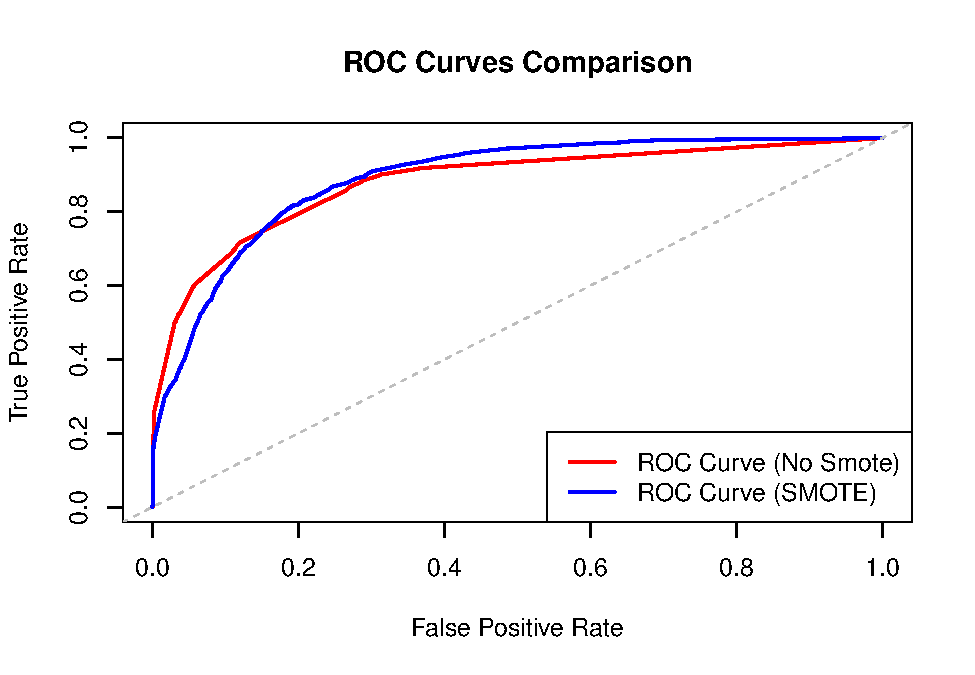
\includegraphics{04-02.2-SurrogateWithSmote_files/figure-latex/unnamed-chunk-3-1.pdf}

The AUC with no SMOTE was 0.8789168. Here, the AUC is 0.8867056, so there was a minor improvement. SMOTE can therefore be beneficial, though it was not very significant in our case.

\section{Upcoming Content}\label{upcoming-content}

We saw SMOTE can be beneficial. Therefore, we change focus and look at other methods of dealing with missing values, in combination with SMOTE. We leave this to the next section.

\section{References}\label{references}

{[}1{]} Fernández, Alberto, et al.~Learning from imbalanced data sets. Vol. 10. No.~2018. Cham: Springer, 2018.

\end{document}
